\documentclass[11pt]{article}
\usepackage[a4paper, margin=1in]{geometry}
\usepackage{graphicx}
\usepackage{float}
\usepackage{amsmath}
\usepackage{csquotes}

\begin{document}
\section*{Task 3: Taylor Rule Approximation of Federal Funds Rate}

The taylor rule presents an interpretation of nominal rates as a function of targets and macroeconomic indicators:

\begin{equation}
    i_t = r^* + \pi_t +
    0.5\underbrace{(\pi_t - \pi^*)}_{\text{Inflation Gap}} +
    0.5\underbrace{(y_t - y^*)}_{\text{Output Gap}}
\end{equation}

\vspace{\baselineskip}

The inflation gap is easily defined as a function of observed inflation and the target.
Output gap is not as clear cut, since GDP potential is not an empirically observable measure.
Common proxies for the potential output are follows:

\begin{description}
    \item[Post-Date Potential Output:] This is an exact measure of potential output, however it is computed after the fact and is open to revisions.
          When faithfully modelling the information set FED had at the time, this measure should not be relied on.
    \item[Trend/Cycle Decomposition:] This method splits the real GDP into a growth term (the trend) and a cyclical fluctuation term (the cycle).
          Output gap is then defined as the cyclical term, which is the gap relative to an \enquote{expected} level.
    \item[Okun's Law:] This method uses the widely accepted relationship between the output and unemployment: $\frac{y_t - y^*}{y^*} = -\alpha(u_t - u^*)$.
          Unemployment measures are more readily available at a given date and revisions are less common compared to real GPD.
          Especially when higher frequency data is used, this method can replace GDP observations, which are often quarterly or annual.
\end{description}

In this exercise, inflation gap is derived from a target of 2\% and FRED's Personal Consumption Expenditure (PCE) index (PCEPILFE).
Output gap is derived from Okun's law with $\alpha=2.0$, using the unemployment rate, and an extrapolation of the quarterly published natural rate of unemplyment.
We assume that the natural unemployment rate cannot move within a quarter.
Finally, $r^*$ is chosen to be 1\%.
The resultingTaylor rule rate compares to the Federal funds rate as follows:

\begin{figure}[H]
    \centering
    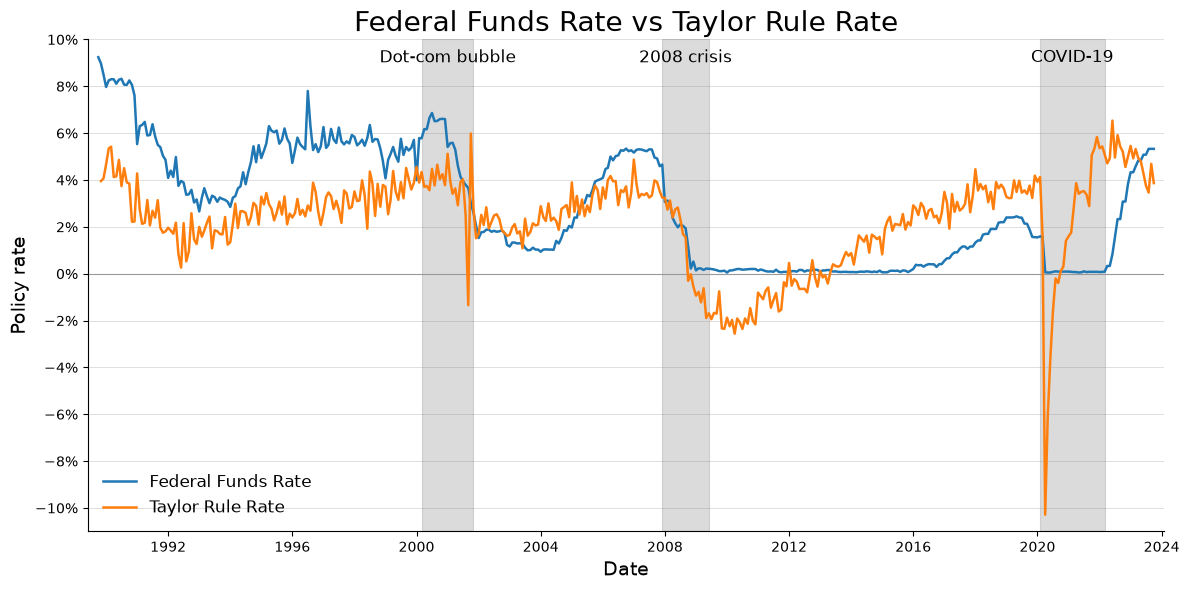
\includegraphics[width=0.8\textwidth]{chart}
    \caption{Taylor Rule and FED Rate over 1989Q3-2023Q3, monthly frequency.}
    \label{fig:taylor_rule}
\end{figure}

\textbf{NOTE:} The steep drop in Taylor rule rate in the COVID-19 shock is partly linked to the output gap being driven by unemployment.
An alternative proxy on real output terms could have been less sensitive to changes in unemployment.

The results show that the Taylor rule is broadly (and/or directionally) consistent with the Federal funds rate.
However, there are notable differences; the highlighted periods mark the time-frames and associated events of the Taylor rule going below 0\%.
Of the three, the dot-com bubble and COVID-19 periods display a steep and momentary shock while the 2008 crisis displays effects that persisted beyond the initial occurence.

\vspace{\baselineskip}

Focusing on 2008 and COVID-19, we observe that both periods display the concept of a \enquote{Zero Lower Bound} (ZLB) or \enquote{Effective Lower Bound} (ELB).
Both notions mark the point at which lowering interest rates further stops being effective.
While ZLB treats 0\% as a hard limit, under ELB small negative rates are thought to remain effective for given economic and behavioral conditions.

\subsection*{Positioning Strategies for Investors}

In scenarios where easing is constrained by the ELB (i.e. Taylor rule suggests below 0\% while FED cannot lower rates further), an investor expecting said scenario to persist can consider positions in longer-duration securities more attractive.
Conversely, when FED is accommodative relative to the Taylor rule (i.e. Taylor rule suggests rates above that of FED's current stance), the investor could steer away from interest rate sensitive instruments or choose short Treasury futures.

\vspace{\baselineskip}

Under the above described broader framework, the initial COVID-19 shock and the 2008 crisis signaled for the long-duration positioning or defensive positioning against falling yields.
Factors such as aggressive QE and fiscal interventions past the initial shock in both cases, however, are factors that can move or flip the conditions.
Particularly, the late response to post-COVID inflationary pressures created an evnironment where an investor anticipating the accommodative stance could have shorted Treasury futures or entered into pay-fixed swaps to capitalize.
\end{document}